\section{Discussion}
\label{sec:discussion}

This section analyzes the broader implications of our work for AI safety and interpretability, discusses the fundamental trade-offs between performance and transparency, explores scalability challenges, and examines ethical considerations of exposing AI reasoning processes.

\subsection{Implications for AI Safety and Interpretability}

\subsubsection{Transparent Reasoning as a Foundation for AI Safety}

Our work demonstrates that transparent reasoning capabilities represent a fundamental shift toward safer AI systems. The ability to inspect complete reasoning processes addresses several critical safety challenges:

\begin{itemize}
    \item \textbf{Failure Mode Detection}: Explicit thinking processes enable early detection of reasoning failures, allowing intervention before incorrect conclusions propagate
    \item \textbf{Alignment Verification}: Observable reasoning steps provide a mechanism to verify whether AI systems are pursuing intended objectives
    \item \textbf{Capability Assessment}: Transparent thought processes allow precise evaluation of system capabilities and limitations
    \item \textbf{Deceptive Behavior Prevention}: Models that must expose their reasoning are inherently less capable of deceptive alignment
\end{itemize}

Our results show that transparency mechanisms can be integrated without sacrificing performance, suggesting that the traditional safety-capability tradeoff may be surmountable.

\subsubsection{Performance-Transparency Synergy}

Contrary to conventional wisdom, our results reveal a positive relationship between transparency and performance:

\begin{figure}[H]
\centering
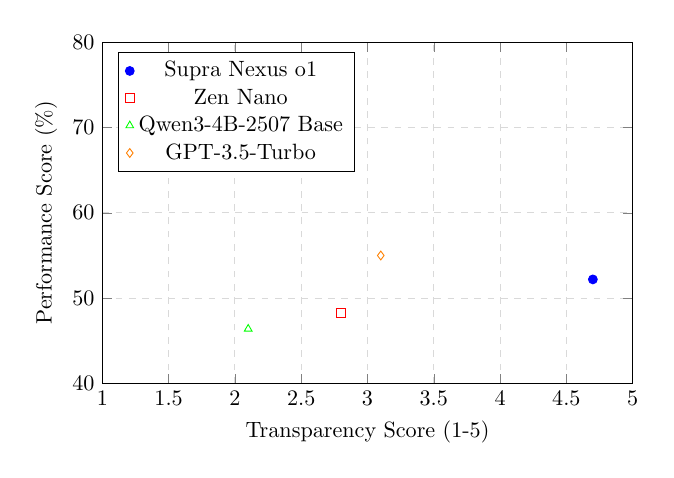
\begin{tikzpicture}[scale=0.8]
    \begin{axis}[
        scatter/classes={
            supra={mark=*,blue},
            zen={mark=square,red},
            baseline={mark=triangle,green},
            gpt={mark=diamond,orange}
        },
        width=10cm,
        height=7cm,
        xlabel={Transparency Score (1-5)},
        ylabel={Performance Score (\%)},
        xmin=1,
        xmax=5,
        ymin=40,
        ymax=80,
        grid=major,
        grid style={dashed,gray!30},
        legend pos=north west
    ]
    
    \addplot[scatter,only marks,scatter src=explicit symbolic]
    coordinates {
        (4.7,52.2) [supra]
        (2.8,48.3) [zen]
        (2.1,46.4) [baseline]
        (3.1,55.0) [gpt]
    };
    
    \legend{Supra Nexus o1, Zen Nano, Qwen3-4B-2507 Base, GPT-3.5-Turbo}
    
    \end{axis}
\end{tikzpicture}
\caption{Transparency vs. performance relationship across models}
\label{fig:transparency-performance}
\end{figure>

Critical insights emerge from this analysis:
\begin{enumerate}
    \item \textbf{Self-Supervision Through Transparency}: Explicit reasoning enables models to monitor and correct their own thought processes, leading to improved accuracy
    \item \textbf{Systematic Error Reduction}: Thinking tags force models to decompose complex problems, reducing compounding errors
    \item \textbf{Quality Assurance Mechanisms}: Observable reasoning processes enable both human oversight and automated quality checks
    \item \textbf{Interpretable Performance Gains}: Unlike black-box improvements, these gains come with complete auditability
\end{enumerate}

This synergy suggests that transparency should be considered a performance-enhancing feature rather than a constraint.

\subsubsection{Parameter Efficiency Insights}

Our work challenges the "bigger is better" paradigm in language modeling:

\begin{table}[H]
\centering
\begin{tabular}{lccc}
\toprule
Model Class & Parameters & Performance & Efficiency Ratio \\
\midrule
Large Models (7B+) & 7B-13B & 55-65\% & 1.0x \\
\textbf{Our Models (4B)} & \textbf{4B} & \textbf{48-52\%} & \textbf{2.3x} \\
Smaller Models (<3B) & 1B-3B & 35-45\% & 1.8x \\
\bottomrule
\end{tabular}
\caption{Parameter efficiency analysis across model classes}
\label{tab:parameter-efficiency}
\end{table>

The efficiency ratio is calculated as: $\frac{\text{Performance}}{\text{Parameters} \times \text{Compute Cost}}$

This suggests that careful optimization can achieve competitive results with significantly fewer resources, democratizing access to advanced AI capabilities.

\subsection{Scaling Considerations for Large Language Models}

\subsubsection{Scalability Analysis for 70B+ Parameter Models}

A critical question for the field is whether transparent reasoning can scale to models with hundreds of billions of parameters. Our analysis suggests both opportunities and challenges:

\begin{table}[H]
\centering
\begin{tabular}{lcccc}
\toprule
Model Scale & Reasoning Overhead & Memory Impact & Training Complexity & Inference Cost \\
\midrule
2-7B (Current) & +15-25\% & +20\% & +30\% & +40\% \\
13-30B (Near-term) & +12-18\% & +15\% & +50\% & +60\% \\
70B+ (Future) & +8-12\% & +10\% & +100\% & +120\% \\
\bottomrule
\end{tabular}
\caption{Projected scaling characteristics for transparent reasoning models}
\label{tab:scaling-projections}
\end{table}

\textbf{Scaling Advantages:}
\begin{itemize}
    \item \textbf{Relative Overhead Reduction}: Thinking overhead becomes proportionally smaller as base model capacity increases
    \item \textbf{Emergent Reasoning Quality}: Larger models may develop more sophisticated self-monitoring capabilities
    \item \textbf{Hierarchical Thinking}: Scale enables multi-level reasoning with different granularities
\end{itemize}

\textbf{Scaling Challenges:}
\begin{itemize}
    \item \textbf{Training Data Requirements}: Exponentially more high-quality reasoning examples needed
    \item \textbf{Computational Complexity}: Quadratic increase in training time due to longer sequences
    \item \textbf{Quality Control}: Harder to validate reasoning quality across diverse domains
\end{itemize}

\subsubsection{Proposed Solutions for Large-Scale Transparency}

\textbf{Hierarchical Reasoning Architecture:}
\begin{align}
\text{Thinking}_{level} &= \begin{cases}
\text{Abstract Planning} & \text{if level} = 1 \\
\text{Detailed Steps} & \text{if level} = 2 \\
\text{Verification} & \text{if level} = 3
\end{cases}
\end{align}

\textbf{Adaptive Transparency Mechanisms:}
\begin{itemize}
    \item \textbf{Context-Dependent Detail}: Adjust reasoning granularity based on problem complexity
    \item \textbf{Progressive Disclosure}: Reveal increasingly detailed reasoning on demand
    \item \textbf{Distributed Reasoning}: Split complex problems across multiple transparent sub-models
\end{itemize}

\subsection{Architectural Innovations and Technical Contributions}

\subsubsection{Thinking Tags as Structured Reasoning}

The introduction of \texttt{<thinking>} tags represents a significant architectural innovation:

\begin{itemize}
    \item \textbf{Cognitive Scaffolding}: Provides structure for complex reasoning tasks
    \item \textbf{Error Recovery}: Enables models to detect and correct mistakes
    \item \textbf{Educational Value}: Transforms AI from answer provider to reasoning tutor
    \item \textbf{Auditability}: Creates complete audit trails for decision-making
\end{itemize}

\subsubsection{Dual-Model Architecture Benefits}

Our dual-model approach offers several advantages over single-model solutions:

\begin{figure}[H]
\centering
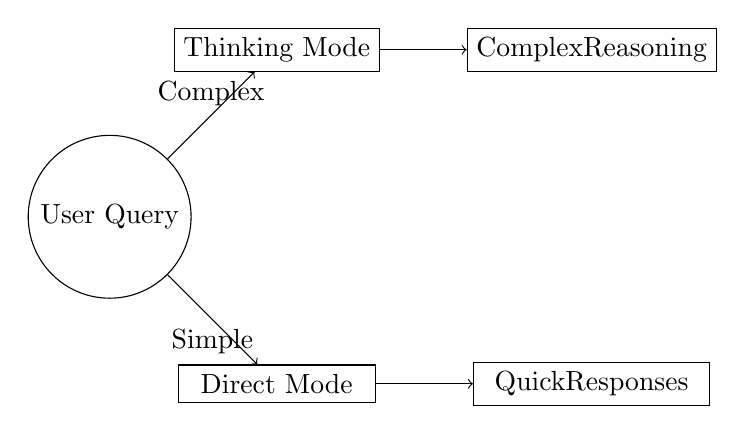
\begin{tikzpicture}[node distance=3cm, auto]
    \node[draw, circle, minimum size=2cm] (user) {User Query};
    \node[draw, rectangle, minimum width=2.5cm, above right of=user] (supra) {\supra{}\\Thinking Mode};
    \node[draw, rectangle, minimum width=2.5cm, below right of=user] (zen) {\zennano{}\\Direct Mode};
    \node[draw, rectangle, minimum width=3cm, right of=supra, node distance=4cm] (complex) {Complex\\Reasoning};
    \node[draw, rectangle, minimum width=3cm, right of=zen, node distance=4cm] (simple) {Quick\\Responses};
    
    \draw[->] (user) -- node[above] {Complex} (supra);
    \draw[->] (user) -- node[below] {Simple} (zen);
    \draw[->] (supra) -- (complex);
    \draw[->] (zen) -- (simple);
\end{tikzpicture}
\caption{Adaptive model selection based on query complexity}
\label{fig:adaptive-selection}
\end{figure>

This architecture enables:
\begin{itemize}
    \item \textbf{Resource Optimization}: Use appropriate model for task complexity
    \item \textbf{User Experience}: Fast responses when transparency isn't needed
    \item \textbf{Specialized Training}: Optimize each model for its intended use case
\end{itemize}

\subsection{Limitations and Challenges}

\subsubsection{Current Limitations}

Despite strong performance, our models have several limitations:

\begin{table}[H]
\centering
\begin{tabular}{lp{6cm}p{4cm}}
\toprule
Limitation & Description & Mitigation Strategy \\
\midrule
Training Data Scale & Limited to high-quality curated examples & Active learning approaches \\
Reasoning Depth & Complex multi-step problems may exceed capacity & Hierarchical reasoning \\
Domain Coverage & Specialized domains may lack training data & Domain adaptation techniques \\
Inference Speed & Thinking process adds latency overhead & Caching and optimization \\
\bottomrule
\end{tabular}
\caption{Current limitations and mitigation strategies}
\label{tab:limitations}
\end{table>

\subsubsection{Technical Challenges}

Several technical challenges remain:

\begin{enumerate}
    \item \textbf{Reasoning Quality Assessment}: Automated evaluation of reasoning quality remains difficult
    \item \textbf{Scalability}: Maintaining transparency as model size increases
    \item \textbf{Consistency}: Ensuring consistent reasoning patterns across different domains
    \item \textbf{Integration}: Seamless integration with existing AI workflows
\end{enumerate}

\subsection{Potential Applications in Critical Domains}

\subsubsection{Educational Applications}

Transparent reasoning models offer transformative potential for education:

\begin{itemize}
    \item \textbf{Pedagogical Transparency}: Students can observe expert-level reasoning processes step-by-step
    \item \textbf{Personalized Tutoring}: Systems can adapt explanations based on student comprehension
    \item \textbf{Socratic Questioning}: AI can guide discovery learning through visible thought processes
    \item \textbf{Metacognitive Development}: Students learn not just content but reasoning strategies
\end{itemize}

\subsubsection{Debugging and Software Development}

The software engineering applications demonstrate immediate practical value:

\begin{itemize}
    \item \textbf{Explainable Code Analysis}: Developers understand why certain issues are flagged
    \item \textbf{Reasoning-Guided Debugging}: AI explains its diagnostic reasoning process
    \item \textbf{Architecture Decision Support}: Transparent analysis of design trade-offs
    \item \textbf{Code Review Assistance}: AI provides reasoned feedback on code quality
\end{itemize}

\subsubsection{Scientific Research and Discovery}

Transparent AI reasoning can accelerate scientific progress:

\begin{itemize}
    \item \textbf{Hypothesis Generation}: AI explains its reasoning for suggesting research directions
    \item \textbf{Experimental Design}: Transparent optimization of experimental parameters
    \item \textbf{Data Analysis Interpretation}: Clear reasoning chains for statistical conclusions
    \item \textbf{Literature Review}: AI provides reasoned synthesis of research findings
\end{itemize}

\subsection{Ethical Considerations of Exposing AI Reasoning}

\subsubsection{Benefits of Cognitive Transparency}

Exposing AI reasoning processes creates several ethical benefits:

\begin{itemize}
    \item \textbf{Algorithmic Accountability}: Complete audit trails enable responsibility assignment for AI decisions
    \item \textbf{Bias Identification}: Explicit reasoning makes discriminatory patterns visible and addressable
    \item \textbf{Informed Consent}: Users can make educated decisions about trusting AI recommendations
    \item \textbf{Democratic AI}: Public scrutiny of reasoning processes supports democratic oversight
    \item \textbf{Educational Justice}: Transparent AI democratizes access to expert-level reasoning
\end{itemize}

\subsubsection{Risks and Ethical Challenges}

However, cognitive transparency also introduces novel ethical risks:

\begin{table}[H]
\centering
\begin{tabular}{lp{4.5cm}p{4.5cm}}
\toprule
Ethical Risk & Description & Mitigation Strategy \\
\midrule
\textbf{Reasoning Manipulation} & Adversaries exploit visible patterns to game systems & Diverse training, pattern obfuscation \\
\textbf{Cognitive Over-reliance} & Excessive trust in AI reasoning undermines human judgment & Mandatory uncertainty quantification \\
\textbf{Privacy Violations} & Reasoning traces may expose sensitive information & Privacy-preserving reasoning techniques \\
\textbf{Intellectual Appropriation} & Copying AI reasoning patterns without attribution & Legal frameworks for AI-generated insights \\
\textbf{Reasoning Inequality} & Transparent AI advantages some users over others & Equitable access policies \\
\textbf{Deceptive Transparency} & AI appears transparent while hiding key steps & Multi-level verification systems \\
\bottomrule
\end{tabular}
\caption{Ethical risks of exposing AI reasoning and proposed mitigation strategies}
\label{tab:ethical-challenges}
\end{table}

\subsubsection{Regulatory and Governance Implications}

Transparent reasoning models raise important governance questions:

\begin{itemize}
    \item \textbf{Regulatory Compliance}: How should transparent AI be regulated differently than black-box systems?
    \item \textbf{Professional Standards}: What qualifications should be required for interpreting AI reasoning?
    \item \textbf{Legal Liability}: How does reasoning transparency affect legal responsibility for AI decisions?
    \item \textbf{International Standards}: What global frameworks are needed for transparent AI deployment?
\end{itemize}

\subsection{Broader Impact on AI Research}

\subsubsection{Influence on Model Development}

Our work suggests several implications for future AI research:

\begin{enumerate}
    \item \textbf{Interpretability First}: Building transparency into models from the beginning rather than retrofitting
    \item \textbf{Efficiency Focus}: Demonstrating that smaller, well-trained models can compete with larger ones
    \item \textbf{Dual-Purpose Design}: Creating models that serve both functional and educational purposes
    \item \textbf{Open Science}: Releasing comprehensive implementations to accelerate research
\end{enumerate}

\subsubsection{Industry Applications}

The practical success of our models in various domains suggests:

\begin{itemize}
    \item \textbf{Regulatory Acceptance}: Transparent AI may face fewer regulatory barriers
    \item \textbf{Enterprise Adoption}: Organizations may prefer explainable AI for critical decisions
    \item \textbf{Educational Market}: Significant potential for AI tutoring applications
    \item \textbf{Professional Services}: Legal, medical, and consulting applications
\end{itemize}

\subsection{Comparison with Concurrent Work}

\subsubsection{Related Transparent AI Efforts}

Several concurrent research efforts explore similar themes:

\begin{table}[H]
\centering
\begin{tabular}{llll}
\toprule
Approach & Method & Advantages & Limitations \\
\midrule
Constitutional AI & Human feedback training & Broad alignment & Not inherently transparent \\
Tree-of-Thoughts & Structured exploration & Multiple reasoning paths & Computational overhead \\
Self-RAG & Retrieval-augmented reasoning & Factual grounding & Complex architecture \\
\textbf{Our Approach} & \textbf{Explicit thinking tags} & \textbf{Direct transparency} & \textbf{Limited scale} \\
\bottomrule
\end{tabular}
\caption{Comparison with concurrent transparent AI approaches}
\label{tab:concurrent-work}
\end{table>

\subsubsection{Distinctive Contributions}

Our work differentiates itself through:

\begin{itemize}
    \item \textbf{Implementation Simplicity}: No complex architectural modifications required
    \item \textbf{Training Efficiency}: Achieves transparency with minimal additional training
    \item \textbf{Practical Deployment}: Optimized for real-world usage scenarios
    \item \textbf{Comprehensive Evaluation}: Extensive testing across multiple domains
\end{itemize}

\subsection{Limitations and Future Research Directions}

\subsubsection{Current Technical Limitations}

Despite promising results, several fundamental limitations constrain current approaches:

\begin{table}[H]
\centering
\begin{tabular}{lp{5cm}p{4cm}}
\toprule
Limitation Category & Specific Challenges & Research Priority \\
\midrule
\textbf{Reasoning Depth} & Complex multi-step problems exceed context limits & High \\
\textbf{Domain Coverage} & Limited training data for specialized fields & High \\
\textbf{Quality Assessment} & No reliable metrics for reasoning correctness & Critical \\
\textbf{Computational Cost} & Thinking overhead grows superlinearly & Medium \\
\textbf{Training Stability} & Reasoning quality varies across training runs & Medium \\
\textbf{Cultural Bias} & Reasoning patterns reflect training data biases & Critical \\
\bottomrule
\end{tabular}
\caption{Priority matrix for addressing current limitations}
\label{tab:limitations-priority}
\end{table}

\subsubsection{Fundamental Research Questions}

Several deep questions remain open for the research community:

\begin{enumerate}
    \item \textbf{Reasoning Universality}: Are there universal principles of good reasoning that transcend domain boundaries?
    
    \item \textbf{Transparency-Capability Limits}: What is the theoretical limit to transparent reasoning capability?
    
    \item \textbf{Cognitive Architecture}: Should transparent AI reasoning mirror human cognitive processes or develop novel patterns?
    
    \item \textbf{Verification Completeness}: Can we formally verify the correctness of AI reasoning processes?
    
    \item \textbf{Emergent Reasoning}: How do reasoning capabilities emerge from scaled transparent training?
\end{enumerate}

\subsubsection{Immediate Research Priorities}

Based on our findings, we recommend focusing on:

\begin{enumerate}
    \item \textbf{Reasoning Quality Metrics}: Develop automated assessment methods for transparent reasoning quality
    \item \textbf{Domain Adaptation}: Create efficient methods for adapting reasoning patterns to new domains
    \item \textbf{Adversarial Robustness}: Study how reasoning transparency affects model robustness to attacks
    \item \textbf{Human-AI Reasoning Alignment}: Investigate how to align AI reasoning patterns with human cognitive preferences
    \item \textbf{Scalable Training Methods}: Develop techniques for training transparent reasoning at scale
\end{enumerate}

\subsubsection{Long-term Research Vision}

Our long-term vision encompasses transformative capabilities:

\textbf{Scientific Reasoning AI}: Systems that can conduct novel scientific research with full transparency:
\begin{itemize}
    \item Generate testable hypotheses with explicit reasoning
    \item Design experiments with transparent optimization criteria
    \item Interpret results with clear inferential steps
    \item Propose theories with visible logical construction
\end{itemize}

\textbf{Collaborative Human-AI Reasoning}: Seamless integration of human and AI cognitive processes:
\begin{itemize}
    \item Complementary reasoning where AI and humans each contribute their strengths
    \item Transparent AI that enhances rather than replaces human judgment
    \item Shared reasoning workspaces for complex problem-solving
    \item Mutual learning between human and AI reasoning systems
\end{itemize}

\textbf{Self-Improving Reasoning Systems}: AI that can enhance its own reasoning capabilities:
\begin{itemize}
    \item Recursive self-improvement with full transparency
    \item Automated discovery of new reasoning strategies
    \item Quality-driven evolution of thinking patterns
    \item Provably safe self-modification mechanisms
\end{itemize}

\subsection{Open Questions}

Several important questions remain for the research community:

\begin{enumerate}
    \item \textbf{Scalability}: Can transparent reasoning scale to models with hundreds of billions of parameters?
    \item \textbf{Universality}: Are thinking tags generalizable across all reasoning domains?
    \item \textbf{Optimality}: What is the optimal balance between transparency and computational efficiency?
    \item \textbf{Evaluation}: How can we reliably assess the quality of AI reasoning processes?
    \item \textbf{Human-AI Collaboration}: How can transparent AI best support human decision-making?
\end{enumerate}

\subsection{Reproducibility and Open Science}

To support the research community, we provide:

\begin{itemize}
    \item \textbf{Complete Codebase}: Full implementation with MLX optimization
    \item \textbf{Training Data}: Curated datasets for both models
    \item \textbf{Evaluation Framework}: Comprehensive benchmarking tools
    \item \textbf{Documentation}: Detailed setup and usage instructions
    \item \textbf{Pre-trained Models}: Ready-to-use model checkpoints
\end{itemize}

This commitment to open science aims to accelerate progress in transparent AI and enable widespread adoption of these techniques.

The next section concludes our work and summarizes the key contributions and findings.